\documentclass[xelatex,ja=standard]{bxjsarticle}
\usepackage[utf8]{inputenc}
\usepackage{amsmath}
\usepackage{amsfonts}
\usepackage{amssymb}
\usepackage{tabularx}
\usepackage{booktabs,dcolumn}
\usepackage{bbm}
\usepackage{natbib}
\setlength{\bibsep}{0.0pt}
\usepackage{graphicx}
\usepackage{setspace}
\usepackage{geometry}
\usepackage{array}
\usepackage[labelformat=simple]{subcaption}
\usepackage{setspace}
\usepackage[titletoc]{appendix}
\usepackage{changepage}
\usepackage{footmisc}
\usepackage{authblk}
\usepackage[disable, colorinlistoftodos,backgroundcolor=white, bordercolor=red, textcolor=red, textsize=tiny]{todonotes}
\usepackage{pdfpages}
\usepackage{subcaption}
\usepackage{comment}
%\usepackage{url} % 文献でのURL表示

\usepackage{lscape}
\usepackage{pdflscape}
\usepackage{rotating}

\usepackage{color}
\definecolor{MyBlue}{rgb}{0,0,0.6}
\usepackage[bookmarks=true,%
bookmarksnumbered=true,%
colorlinks=true,%
linkcolor=MyBlue,%
citecolor=MyBlue,%
filecolor=MyBlue,%
urlcolor=MyBlue%
]{hyperref}

\onehalfspacing
\bibpunct{(}{)}{;}{a}{}{;}
\geometry{top=2cm, bottom=2cm, left=3cm, right=3cm}
\newcolumntype{Z}{>{\centering\arraybackslash}X}
\abovecaptionskip=-2pt
\setlength{\marginparwidth}{2cm} % for todonotes
\usepackage{fontspec}
\usepackage{underscore}
\usepackage[T1]{fontenc}
  
\setCJKsansfont[Path = ../../../\detokenize{01_admin}/preamble/tex/fonts/,
BoldFont = HaranoAjiGothic-Bold.otf]
{HaranoAjiGothic-Regular.otf}

\setCJKmainfont[Path = ../../../\detokenize{01_admin}/preamble/tex/fonts/,
BoldFont = HaranoAjiMincho-Bold.otf]
{HaranoAjiMincho-Regular.otf}

\usepackage{threeparttable}
\usepackage{float}



\title{朝ごはんと成績に統計的関係があるか \\ -- Peanutsのデータを用いて -- \thanks{本レポートは、データサイエンスの授業において、R/RStudio、Git/GitHub、LaTeX/Overleafを組み合わせて、再生可能なプログラミングとレポート文書作成の例として作成したものである。レポートの書式としては、あくまで内部資料として作成しており、外部向けの論文の形式を取っていない。また、Peanutsの設定は全て仮想である。}}

\author{Charlie Schultz
\thanks{Department of Comics. Email: cshultz@comics.edu}  \ \  Chishio Furukawa
\textsuperscript\thanks{Department of Economics. Email:cfurukawa@economics.ac.jp}}

%\date{\today}
\date{March, 1990}


\begin{document}
\renewcommand\footnotelayout{\small}
\sffamily\mdseries

\maketitle

\vspace{-10pt}\begin{abstract}
\begin{spacing}{1}
\noindent 
Peanutsの登場キャラクターたちは、自分たちの経験に基づき「好きな朝ごはんを食べることが、学校の成績につながる」と考えている。本レポートでは、この統計的根拠を探索し、以下の結果を得た。(1)朝ごはんに``pancake''を食べることは、小テストの成績と強く相関はしていなかった。(2)Snoopyが``corn flake''の代わりに``dog flake''ばかり買ったときには「朝ごはんに``dog flake''を食べ、アレルギーで勉強に集中できなかった」とCharlieとSallyは言っているが、これについては整合的な根拠が示された。\\

\end{spacing}
\end{abstract}

\newpage

\section{はじめに}

\subsection{背景} 

この統計分析は、朝ごはんと成績の関係性を吟味することを目的としている。CharlieやLucieらは、「おいしい朝ごはんを食べることが学校の成績に欠かせない」と信じている。特に、pancakes(和製英語:ホットケーキ)は好物で、トーストやオートミールよりも、pancakesをもっと食べたいと考えている。学術的にも、朝ごはんを食べることが学校の成績と相関していると言われている\citep{Furuse2020b}。

\subsection{問い}

本レポートでは、James Elementary Schoolと、それぞれの朝ごはんの記録のデータを結び付けて、次の2つの問いについて考える。

\begin{enumerate}
\item pancakeを食べることは、学校の成績に相関しているだろうか。
\item 「dog flakesを食べることによって、勉強に集中できず、成績が悪くなった」という主張は、統計的に整合的だろうか。
\end{enumerate}

\subsection{記述統計}

まず、統計分析をはじめる前に、登場キャラクターが、どのような朝ごはんを食べているかをまとめよう。

\begin{table}[!h]
\centering
\begin{tabular}[t]{lrr}
\toprule
breakfast\_renamed & count & frequency\\
\midrule
cereal & 292 & 0.33\\
dog flakes & 6 & 0.01\\
no breakfast & 41 & 0.05\\
oatmeal & 206 & 0.23\\
pancakes & 178 & 0.20\\
\addlinespace
toast & 172 & 0.19\\
\bottomrule
\end{tabular}
\end{table}

(この表においては、キャラクターの記録した名前を整理してある。例: corn flake $\rightarrow$ cereal、など)

\textbf{所感:}
\begin{itemize}
\item もっともよく食べるものは、cerealやtoastなどである。
\item pancakeを食べることは稀であり、特別だということが分かる。
\item dog flakesを食べなくてはいけないことは数回しかなかった。
\end{itemize}

\section{分析} 

\subsection{pancakesと成績の関係}
\subsubsection{散布図}
まず探索的な分析として、重要な変数の相関などを知るために散布図を描くことが効果的である。図\ref{fig:img1}は、学生ごとに色を変え、ある月のうちのpancake率と成績をプロットしたものである。

\begin{figure}[h]
\centering
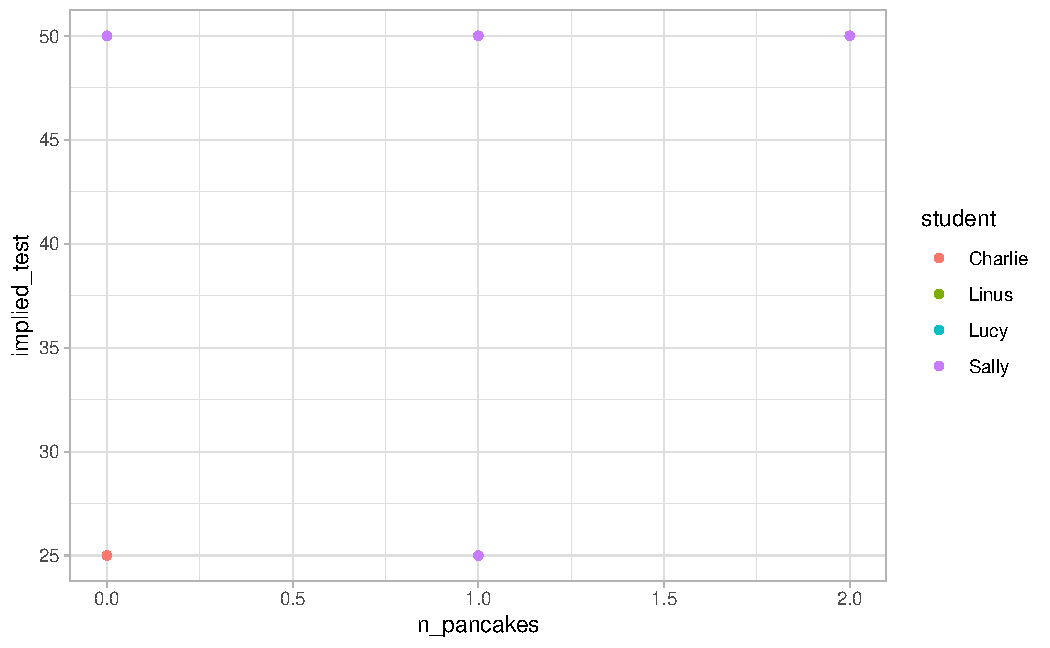
\includegraphics[width=12cm]{04_analyze/pancakes_study/figure/pancakes_study.pdf}
\label{fig:img1}
\caption{pancakeと成績の散布図}
\end{figure}

(この図\ref{fig:img1}は、ggplot2パッケージを用いて作成した「探索的図画」である。例えば、変数名やタイトルなどを調整していない。)

\textbf{所感}
\begin{itemize}
\item 全体としては、pancakeと成績の間に弱い相関があるように見える。
\item しかし、この相関は、学生の間の関係であって、それぞれの学生に着目をすれば「pancakeをよく食べた月の方が成績がよかった」というわけではないようである。
\end{itemize}

\subsubsection{回帰分析}
この散布図で見られた関係を、回帰分析によってより厳密に考えたいと思います。以下の回帰式を推定したいとします。

\begin{equation}
Test_{it} = \beta_0 + \beta_{1} \text{frac(pancakes)}_{it} + f_{i} + \varepsilon_{it}

\end{equation}

\begin{itemize}
\item $Test_{it}$は、数学と英語の平均の点数
\item frac(pancakes)$_{it}$ は、学生$i$にとって月$t$に食べたpancakeの率
\item $f_i$ は、学生$i$のダミー変数であり、固定効果を推定するためにある
\end{itemize}

ここで、関心のある推定量は$\beta_{1}$であり、pancake率が上昇することによって、成績が何ポイント改善するかを表している。

\begin{table}

\caption{Initial regressions}
\centering
\begin{threeparttable}
\begin{tabular}[t]{lcc}
\midrule\midrule
\multicolumn{1}{c}{ } & \multicolumn{1}{c}{(1)} & \multicolumn{1}{c}{(2)} \\
\cmidrule(l{3pt}r{3pt}){2-2} \cmidrule(l{3pt}r{3pt}){3-3}
  & OLS & FE\\
\midrule
frac(pancakes) & \num{141.58} & \num{89.02}\\
 & (\num{20.80}) & (\num{117.94})\\
Constant & \num{42.61} & \\
 & (\num{4.84}) & \\
\midrule
Clustering & Y & Y\\
Num.Obs. & \num{25} & \num{25}\\
R2 & \num{0.373} & \num{0.388}\\
R2 Adj. & \num{0.346} & \num{0.227}\\
\midrule\midrule
\end{tabular}
\begin{tablenotes}
\item \textit{Note: } 
\item Heteroskedasticity-robust standard errors clustered at students level are reported in the parenthesis.
\end{tablenotes}
\end{threeparttable}
\end{table}


この回帰分析の推定結果が、表1にまとめられている。

\textbf{所感:}
\begin{itemize}
\item OLSによって、全体の相関を見ると、ある程度の相関が見られる。
\item FEによって、個々人の学生にとっての相関を見ると、その相関はほとんどなくなっている。
\end{itemize}

(ここでは、統計的有意水準は示していない。これは、帰無仮説検定によってのみ結論の判断をすることを避けるためである。)

\subsection{dog flakesと成績の関係}

CharlieとSallyは、Snoopyがdog flakesのみしか朝ごはんに買っていなかったときがあったため、アレルギーで勉強をできなかった、と言っている。そこで、dog flakesを食べた月の試験は、実際にBrown兄弟のみ成績の低下が見られたかどうかを検証する。

\begin{figure}[h]
\centering
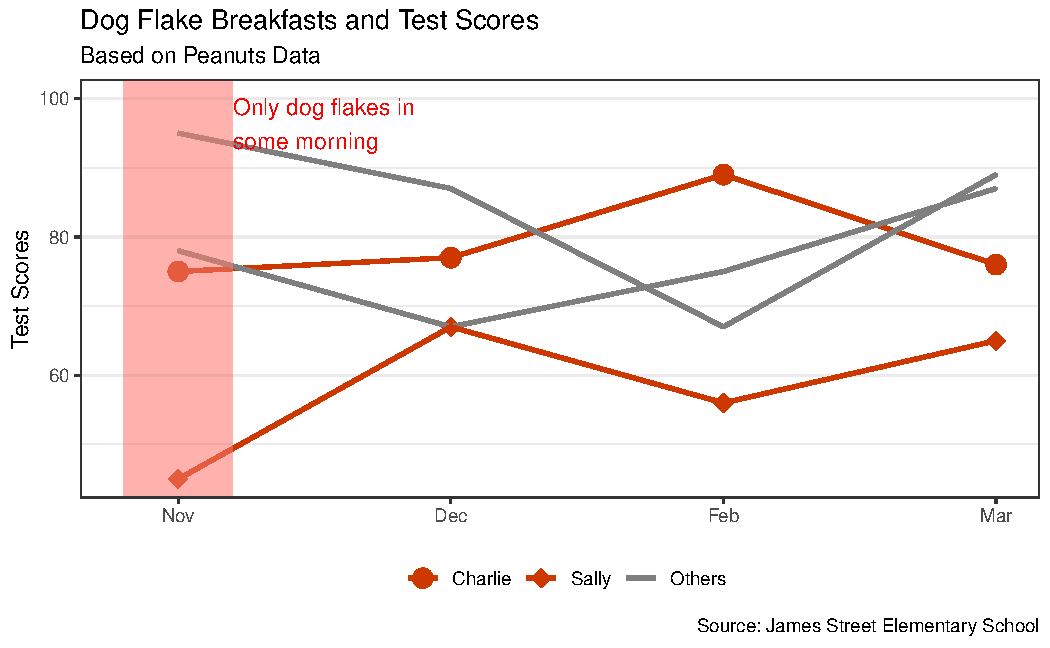
\includegraphics[width=12cm]{00_cover/dogflakes.pdf}
\label{fig:img2}
\caption{dog flakesショックとBrown兄弟の成績}
\end{figure}

(この図\ref{fig:img2}は、ggplot2パッケージを用いて作成した「発表向け図画」である。軸の名称やタイトル、またキャプションなどをつけ、また配色もマニュアルで調整している。)

\textbf{所感:}
\begin{itemize}
\item 他の学生と比べ、dog flakeを食べた月と、その次の月の成績が低下していることが見られる。
\item サンプル数が少ないため統計的検定をすることは難しいかもしれないが、CharlieとSallyの主張は正しい可能性が示唆された。
\item pancakeに関する分析は、コントロール変数などをあまり入れられていないこともあり、因果的解釈が難しい。これに対して、もし「Snoopyがdog flakesのみを買ったこと」がその他の諸要因とは関係がなかった「外生的ショック」と考えることが妥当ならば、dog flakesの項かとして捉えることができそうであ。

\end{itemize}

\newpage

\bibliographystyle{econ} 
\bibliography{06_literature/00_bibliography/literature}
%\bibliography{example}


\end{document}